%%%%%%%%%%%%%%%%%%%%%%%%%%%%%%%%%%%%%%%%%%%%%%%%%%%%
% Packages and commands
%%%%%%%%%%%%%%%%%%%%%%%%%%%%%%%%%%%%%%%%%%%%%%%%%%%%
\documentclass[12pt,letterpaper]{uncdissertation}

\usepackage{uncdissertation} 





%%%%%%%%%%%%%% begin doc %%%%%%%%%%


\begin{document}
\thesistitle{THREE ESSAYS ON ...}

\thesisauthor{Author} 
\thesisadvisor{Committee chair}
\thesisreadera{Committee member 1} 
\thesisreaderb{Committee member 2} 
\thesismembera{Committee member 3}
\thesismemberb{Committee member 4} 


\thesismaketitle 
\thesismakecopyright


\doublespacing
% % % % % % % % % % % % % % % % % % % % % % % %
% Abstract
% % % % % % % % % % % % % % % % % % % % % % % %


\begin{abstract}
Influencers and digital platforms are reshaping consumer decision-making and firms’ strategies. My dissertation studies the strategic interactions between firms, influencers, consumers, and digital platforms.

The first three essays take the perspective of the firm. In Essay 1, I develop a conceptual framework to integrate influencer marketing into marketing strategy. Drawing from interviews with 15 marketing managers, I identify the challenges managers face in the design and execution of influencer marketing strategy and develop a framework to help managers select the right portfolio of influencers for each stage of the customer decision-making journey.

In Essay 2, I study how duopoly firms optimally choose influencer effort types and product pricing strategies. The model extends horizontal and vertical differentiation thinking to the influencer context. I examine when firms should engage influencers in effort overflow—educating consumers about the product category—and when they should engage influencers in effort variety—diversifying content formats to combat creativity fatigue. My findings indicate that effort overflow increases firm profits by alleviating influencer competition in effort levels, while effort variety intensifies such competition.

In Essay 3, I employ a Bayesian persuasion perspective to study how influencers strategically design their reviews in a market where early adopters’ reviews contribute to information dissemination. I find that the optimal influencer strategy depends on the valence and informativeness of early adopters’ reviews, and I characterize the conditions under which the seller should use non-performance-based contracts or sales-based commissions. These results highlight the influencer’s role as a strategic information intermediary who corrects information distortions to facilitate product-consumer matching.



Together, these essays provide a deeper understanding of how information, influencers, and algorithms interact in shaping consumer behaviors and firm decisions in the digital marketing environment.
\end{abstract}


% % % % % % % % % % % % % % % % % % % % % % % %
% optional dedication and acknowledgments
% % % % % % % % % % % % % % % % % % % % % % % %

%\begin{dedication}
%\begin{center}
%\textit{Your dedication goes here.}
%\end{center}
%\end{dedication}

    \begin{acknowledgments}


In the process of writing this dissertation...


\end{acknowledgments}



%%%%%%%%%%%%%%%%%%%%%%%%%%%%%%%%%%%%%%%%%%%%%%%%%%%%
% Table of contents and lists
%%%%%%%%%%%%%%%%%%%%%%%%%%%%%%%%%%%%%%%%%%%%%%%%%%%%
\newpage
\begin{spacing}{1}
\begingroup
\renewcommand*{\addvspace}[1]{}
\hyphenpenalty=10000
\exhyphenpenalty=10000
\pretolerance=10000
\tolerance=2000
\emergencystretch=1em
\tableofcontents
\newpage
\addcontentsline{toc}{chapter}{LIST OF TABLES}
\listoftables
\newpage
\addcontentsline{toc}{chapter}{LIST OF FIGURES}
\listoffigures
\endgroup
\end{spacing}

%%%%%%%%%%%%%%%%%%%%%%%%%%%%%%%%%%%%%%%%%%%%%%%%%%%%
% Begin manuscript
%%%%%%%%%%%%%%%%%%%%%%%%%%%%%%%%%%%%%%%%%%%%%%%%%%%%
\begin{doublespace}
\cleardoublepage
\pagenumbering{arabic}

%%%%%%%%%%%%%%%%%%%%%%%%%%%%%%%%%%%%%%%%%%%%%%%%%%%%
% Chapter 1
%%%%%%%%%%%%%%%%%%%%%%%%%%%%%%%%%%%%%%%%%%%%%%%%%%%%
\begin{singlespace}
\chapter{TITLE OF CHAPTER 1}
\end{singlespace}\label{chap1}

\section{Introduction}
This sample chapter includes placeholder prose and citations commonly used in economics doctoral writing. Classic problems of information asymmetry are often introduced with \citet{akerlof1970lemons}, while dynamic reputation and equilibrium selection are commonly linked to \citet{krepswilson1982}. Broader treatments of institutions and long-run development include \citet{acemoglu2001colonial}.

\clearpage
\begin{landscape}
\thispagestyle{empty}
\landscapepageno
\noindent
\begin{minipage}[c][6.35in][c]{9in}
\centering
\huge A Large Wide Table
\vspace{0.3em}
\captionsetup{type=table,hypcap=false}
\captionof{table}[Sample Literature Mapping Table]{Sample Literature Mapping Table}
\label{tab:table1_conceptual}
\end{minipage}
\end{landscape}
\clearpage




%%%%%%%%%%%%%%%%%%%%%%%%%%%%%%%%%%%%%%%%%%%%%%%%%%%%
% Chapter 2
%%%%%%%%%%%%%%%%%%%%%%%%%%%%%%%%%%%%%%%%%%%%%%%%%%%%
\begin{singlespace}
\chapter{TITLE OF CHAPTER 2}\label{chap2}
\end{singlespace}





\section{Introduction}

	\begin{figure}[htbp]
    
\includegraphics[width = 0.8\textwidth]{images/UNC_logo.png}
		\caption{UNC is good}
		\label{fig: UNC}
	\end{figure}
	


%%%%%%%%%%%%%%%%%%%%%%%%%%%%%%%%%%%%%%%%%%%%%%%%%%%%
% Chapter 3
%%%%%%%%%%%%%%%%%%%%%%%%%%%%%%%%%%%%%%%%%%%%%%%%%%%%
\begin{singlespace}
\chapter{TITLE OF CHAPTER 3 IS GENERATED BY AI SO IT IS EXTRAORDINARILY LONG}\label{chap3}
\end{singlespace}


\section{Illustration}
    
	\begin{table}[htbp]
		\centering
		\small
		\renewcommand{\arraystretch}{1.2}
		\begin{tabularx}{\textwidth}{|c|Y|Y|}
			\hline
			& \textbf{Influencer} & \textbf{Early adopter} \\
			\hline
			\textbf{Product reviews} & Two-sided review &  Perfect good (bad) review \\
			\hline
			\textbf{Strategic orientation} &  Strategic& Non-strategic \\
			\hline
			\textbf{Objective functions} 
			& Maximize a mix of consumer welfare and sales commissions
			& No objective \\
			\hline
			\textbf{Decision variables} 
			& ($\mu_s, p_s), s\in \{G,M,B\}$ 
			& No decision variable\\
			\hline
		\end{tabularx}
		\caption{Comparison of the two sources driving consumer learning}
		\label{tab:organic_influencer_influencer_lead_user}
	\end{table}
	
	
	
	
	
	\subsection{Timeline of the actions}\label{sec: timeline}
	The timeline of the game is summarized in Figure \ref{fig: timeline}. Given the presence of the early adopter, a seller endogenously decides whether to use an influencer during product launch. Conditional on using an influencer, the seller designs the influencer contract with foresight into the mapping of the realized product match to the influencer's review---i.e., the influencer's reputation. The influencer then commits to an information structure. 
   After the product-consumer match is realized for the influencer and the early adopter,  they post their reviews. The seller then sets a profit-maximizing launch price. After seeing the formal launch price, consumers update their beliefs about the product-consumer match and decide whether to purchase the product. We use backward induction to arrive at the market-clearing outcomes. 




	\begin{figure}[htbp]
		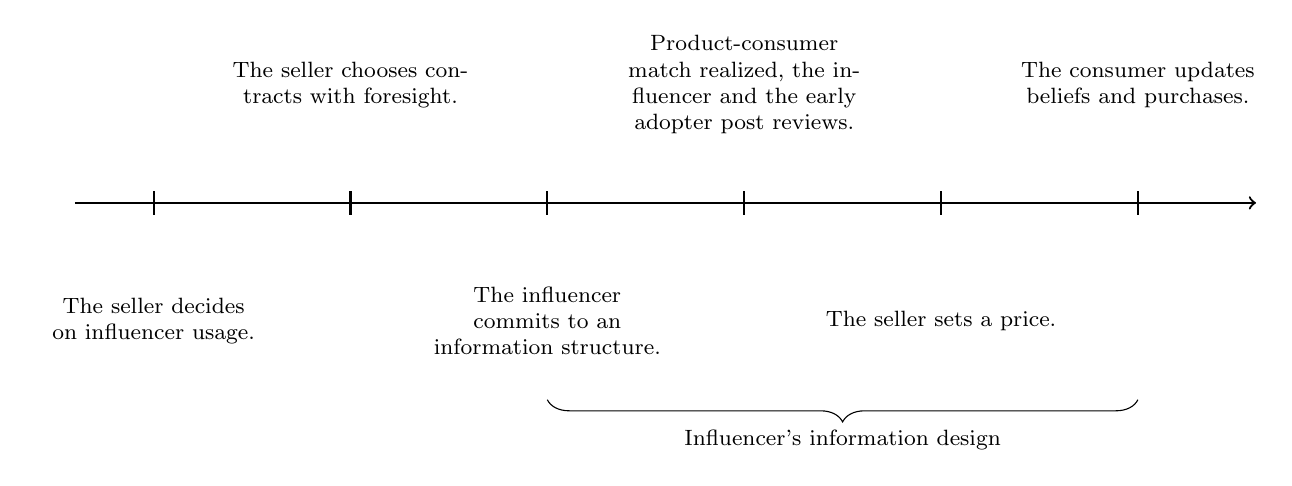
\begin{tikzpicture}[scale=5]
			\footnotesize
			%%%%%%%%%the first line%%%%%%
			%%%%%%%%%%left panel graph*****************
			%\node at (-0.3, 2.45) {$t$};
			\node[align=center,text width=3cm] at (0, 2.2) {The seller decides on influencer usage.};
			
			\node[align=center, text width=3cm] at (0.5, 2.8) {The seller chooses contracts with foresight.};
			
			\node[align=center, text width=3cm] at (1, 2.2) {The influencer commits to an information structure.};
			
			\node[align=center,text width=3cm] at (1.5, 2.8) {Product-consumer match realized, the influencer and the
				early adopter post reviews.};
			\node[align=center,text width=3cm] at (2, 2.2) {
			The seller sets a price.};
			
			\node[align=center,text width=3cm] at (2.5, 2.8) {The consumer updates beliefs and purchases.};
			
			
			\draw [thick, ->] (-0.2,2.5) -- (2.8,2.5);
			\draw [thick] (0,2.47) --(0,2.53);
			\draw [thick] (0.5,2.47) --(0.5,2.53);
			\draw [thick] (1,2.47) --(1,2.53);
			\draw [thick] (1.5,2.47) --(1.5,2.53);
			\draw [thick] (2,2.47) --(2,2.53);
			\draw [thick] (2.5,2.47) --(2.5,2.53);
			
			
			% Add a bracket under timeline between 1 and 7
			\draw[decorate,decoration={brace,amplitude=8pt,mirror}] (1,2) -- (2.5,2) node[midway,below,yshift=-8pt]{Influencer's information design};
			
		\end{tikzpicture}
		\caption{Timeline of the game}
		\label{fig: timeline}
	\end{figure}
	

	
	






%%%%%%%%%%%%%%%%%%%%%%%%%%%%%%%%%%%%%%%%%%%%%%%%%%%%
% Appendix A
%%%%%%%%%%%%%%%%%%%%%%%%%%%%%%%%%%%%%%%%%%%%%%%%%%%%
\titlespacing{\chapter}{0pt}{-.375in}{12pt} %This changes top margin for first page of Appendices and Bibiography to 1", the first pages of the chapters have a 2" top margin

\appendix
\renewcommand{\appendixname}{APPENDIX}
\renewcommand{\cftchappresnum}{APPENDIX\ }
\renewcommand{\cftchapaftersnum}{:\ }
\settowidth{\cftchapnumwidth}{APPENDIX D:\ }

\begin{singlespace}
\refstepcounter{chapter}
\phantomsection
\chapter*{APPENDIX \thechapter: Appendix for Chapter 1}
\addcontentsline{toc}{chapter}{APPENDIX \thechapter: Appendix for Chapter 1}
\end{singlespace}
\section{Technical Details}
This is the appendix for Chapter 1. 

\begin{singlespace}
\refstepcounter{chapter}
\phantomsection
\chapter*{APPENDIX \thechapter: Appendix for Chapter 2}
\addcontentsline{toc}{chapter}{APPENDIX \thechapter: Appendix for Chapter 2}
\end{singlespace}
\input{appA_Chapter2}

\begin{singlespace}
\refstepcounter{chapter}
\phantomsection
\chapter*{APPENDIX \thechapter: Appendix for Chapter 3}
\addcontentsline{toc}{chapter}{APPENDIX \thechapter: Appendix for Chapter 3}
\end{singlespace}
\input{appA_Chapter3}

%%%%%%%%%%%%%%%%%%%%%%%%%%%%%%%%%%%%%%%%%%%%%%%%%%%%
% References
%%%%%%%%%%%%%%%%%%%%%%%%%%%%%%%%%%%%%%%%%%%%%%%%%%%%

\clearpage
\addcontentsline{toc}{chapter}{REFERENCES}
\begin{singlespace}
\bibliographystyle{chicago}
\bibliography{Bibliography}
\end{singlespace}



%%%%%%%%%%%%%%%%%%%%%%%%%%%%%%%%%%%%%%%%%%%%%%%%%%%%
% End the document
%%%%%%%%%%%%%%%%%%%%%%%%%%%%%%%%%%%%%%%%%%%%%%%%%%%%
\end{doublespace}
\end{document}